\chapter{Background}
\label{chap:bg}
In this chapter, we first introduce the generative probability topic.
They are the basic of our framework.

\section{Transformer}
\label{section:transformer}
The Transformer is a model proposed by Vaswani, Ashish et al. in 2017~\cite{vaswani2017attention}  that uses the attention mechanism to increase the speed of model training. Compared with recurrent networks eg., Long short-term memory (LSTM), the Transformer can model long dependencies between input sequence elements and support parallel processing of sequence. and get higher both accuracy and performance than the popular RNN recurrent neural network. It mainly consists of two parts: the Encoder and Decoder. The structure of the Transformer is shown below as Fig.~\ref{fig:transformer}.

The transformer model  was first applied to a wide range of language tasks such as text classification, machine translation, and question answering, and demonstrated exemplary performance. The breakthrough from Transformer network in the field of natural language processing (NLP) has aroused great interest in the computer vision community, meanwhile the Transformer model and its variants have been successfully applied to the various fields of computer vision, such as image recognition, object detection, segmentation, image super-resolution, video understanding, image generation and so on. 

\begin{figure}[!htbp]
	\centering
	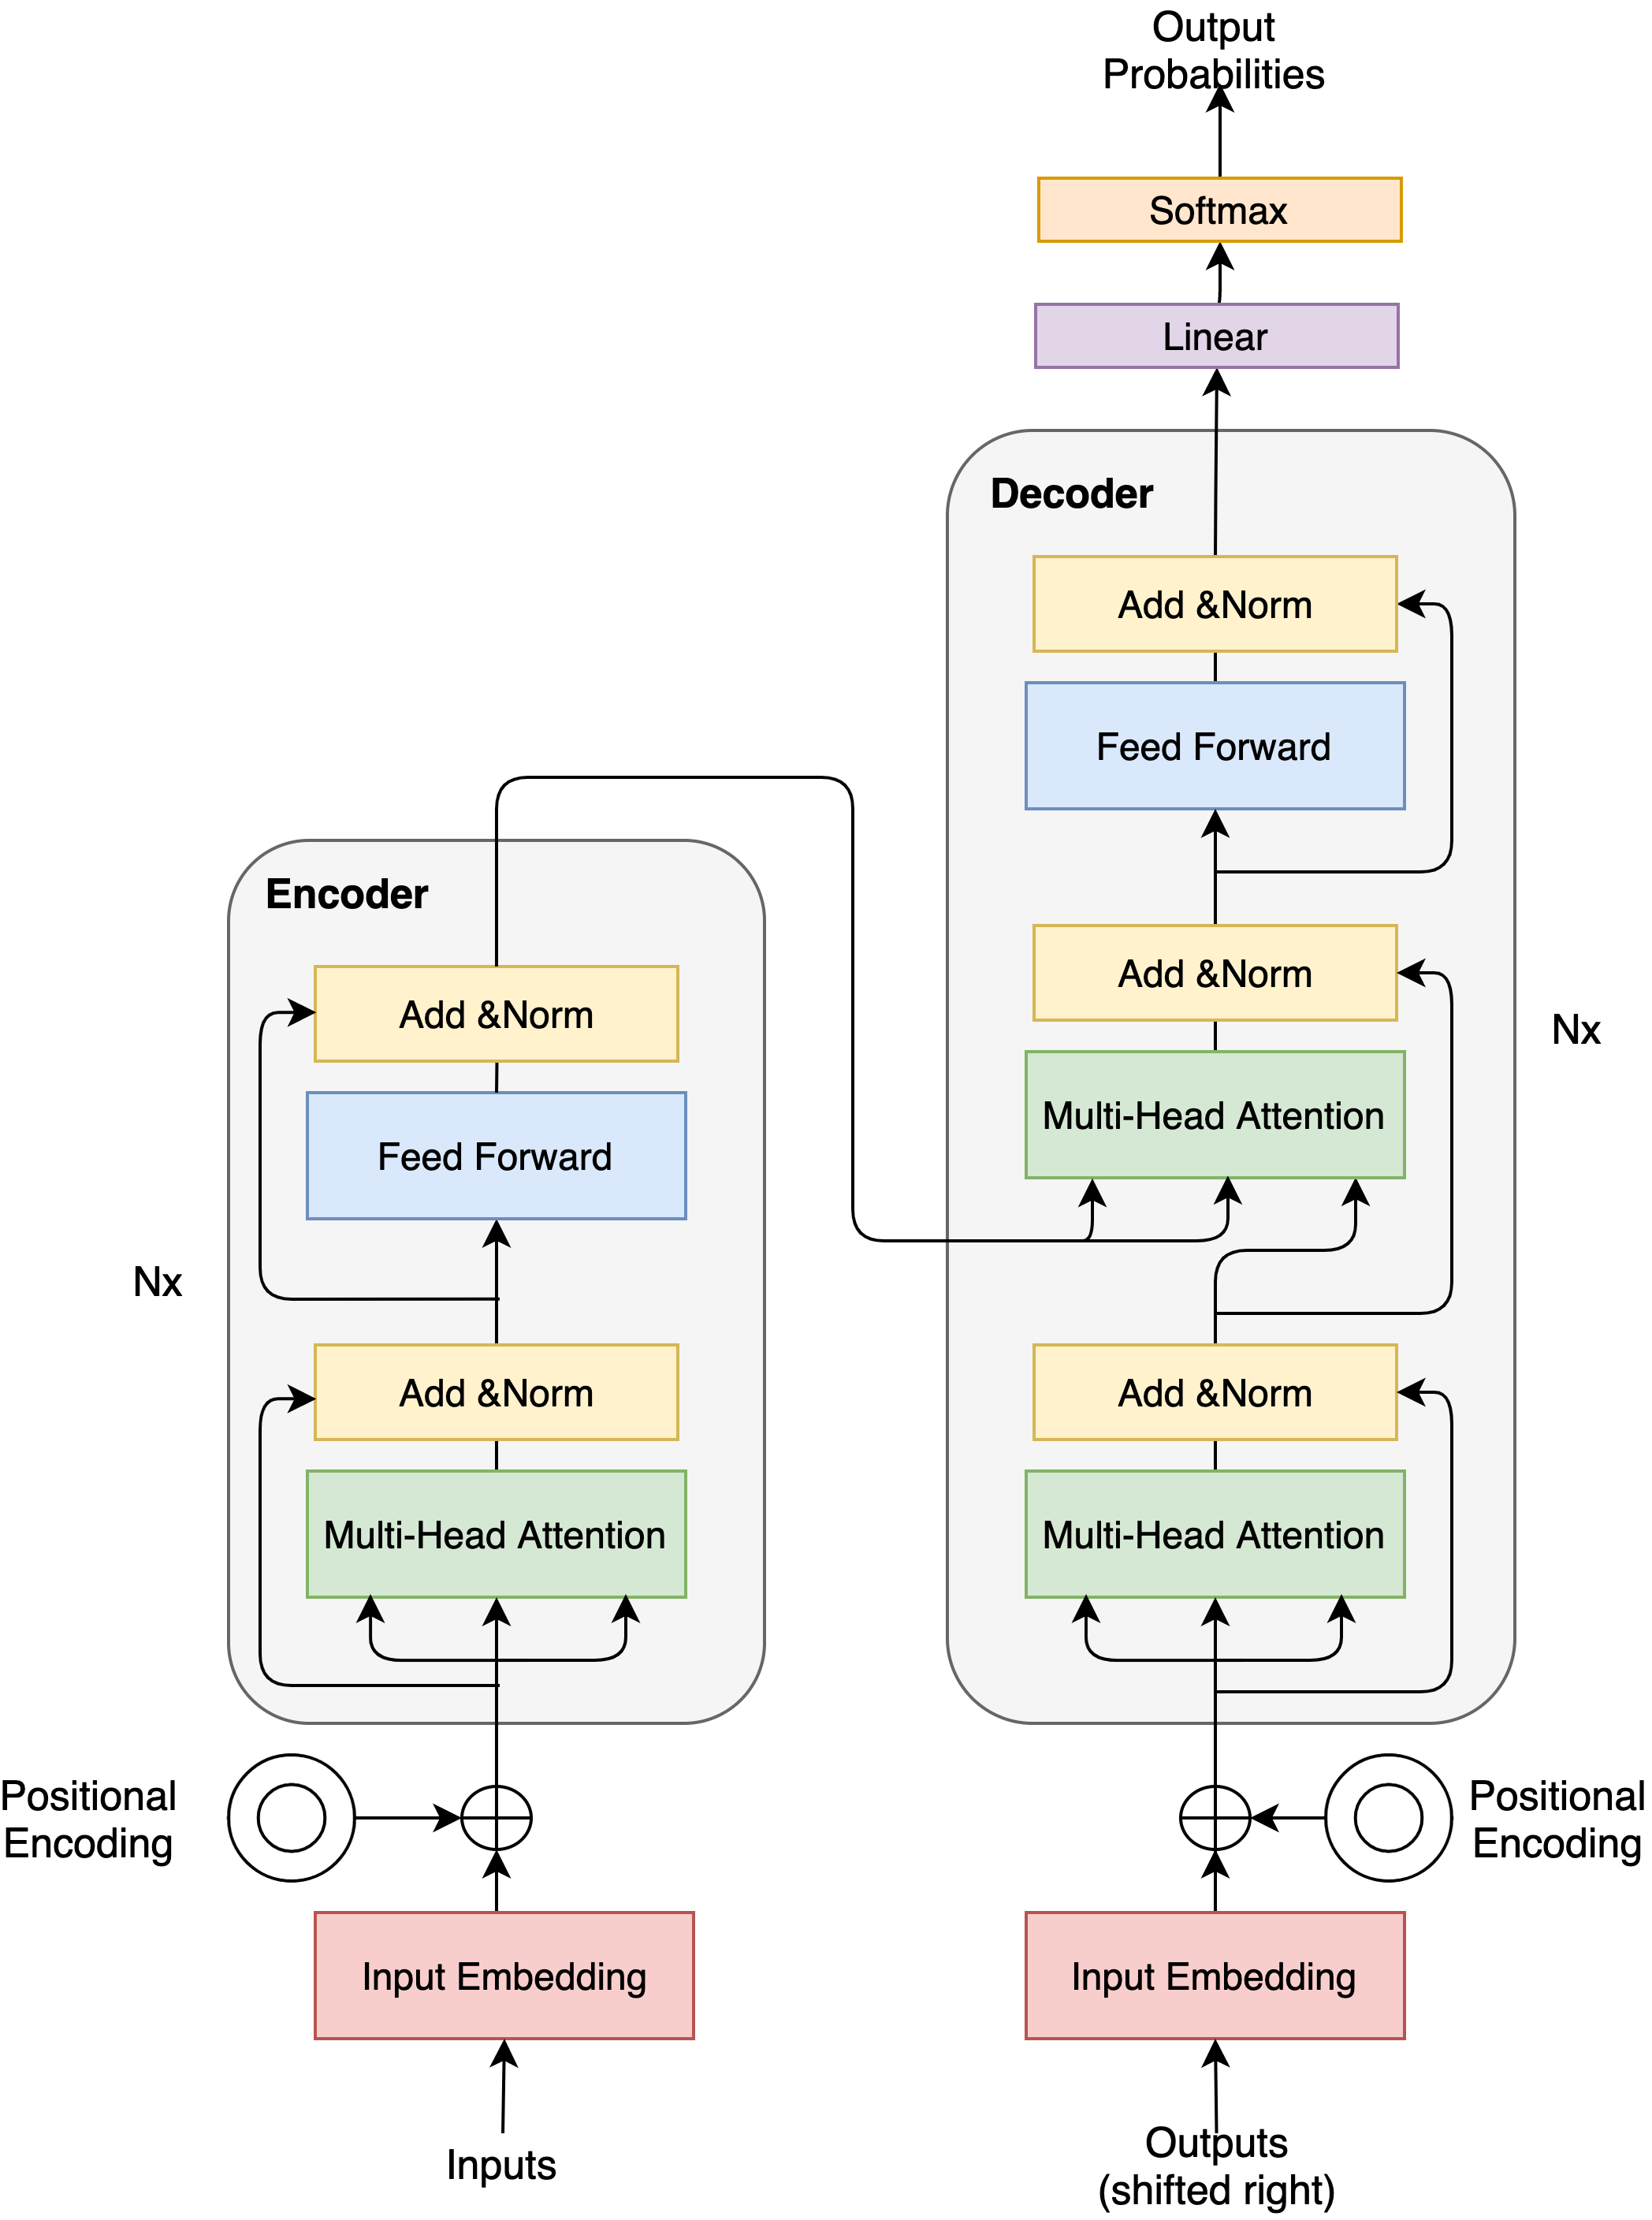
\includegraphics[width = 0.5 \textwidth]{figures/transformer.png}
	\caption[The Transformer - model architecture]
	{ The Transformer - model architecture.~\cite{vaswani2017attention}.}
	\label{fig:transformer}
\end{figure}

\subsection{Self-Attention}
An attention function can be described as mapping a query and a set of key-value pairs to an output, where the query, keys, values, and output are all vectors. The output is computed as a weighted sum of the values, where the weight assigned to each value is computed by a compatibility function of the query with the corresponding key.

From the following table~\ref{tab:complexity_compare}, we can know that self attention has a great improvement for longer sequences. For image data, we can think of it as a longer sequence, and it would be better to optimize it.
\begin{table}[!htbp]
	\resizebox{\textwidth}{15mm}{
	\begin{tabular}{cccc}
		\hline
		Layer Type                  & Complexity per Layer & Sequential Operations & Maximum Path Length \\ \hline
		Self-Attention              & $ O(n2\cdot d)  $           &$  O(1)  $                 & $ O(1)  $               \\
		Recurrent                   & $ O(n2\cdot d) $            & $ O(n)  $                 & $ O(n)  $               \\
		Convolutional               & $O(k\cdot n\cdot d^2)$       & $O(1) $              & $O(log_k(n)$)         \\
		Self-Attention (restricted) & $ O(r\cdot  n \cdot d) $         & $ O(1)  $                 & $ O(n/r)  $             \\ \hline
	\end{tabular}}

\caption[Compare between Self-Attention and Convolutional ]
{ Maximum path lengths, per layer complexity and minimum number of sequential operations for different layer types. n is the sequence length, d is the representation dimension, k is the kernel size of convolutions and r the size of the neighborhood in restricted self-attention. ~\cite{vaswani2017attention}.}
	\label{tab:complexity_compare}
\end{table}

There are three very important vectors in attention, query, key, and value. For self- attention, these three vectors are obtained by multiplying the same vector by different ma- trices(see Fig. 3.3).
An attention function can be described as mapping a query and a set of key-value pairs to an output. The input consists of queries and keys of dimension d , and values of dimension d ,
softmax function to obtain the weights on the values.


\begin{equation}
	Attention(Q,K,V)=softmax(\frac{QK^T}{\sqrt{d_K}})V
	\label{equ:self_attention}
\end{equation}


\begin{figure}[!htbp]
	\centering
	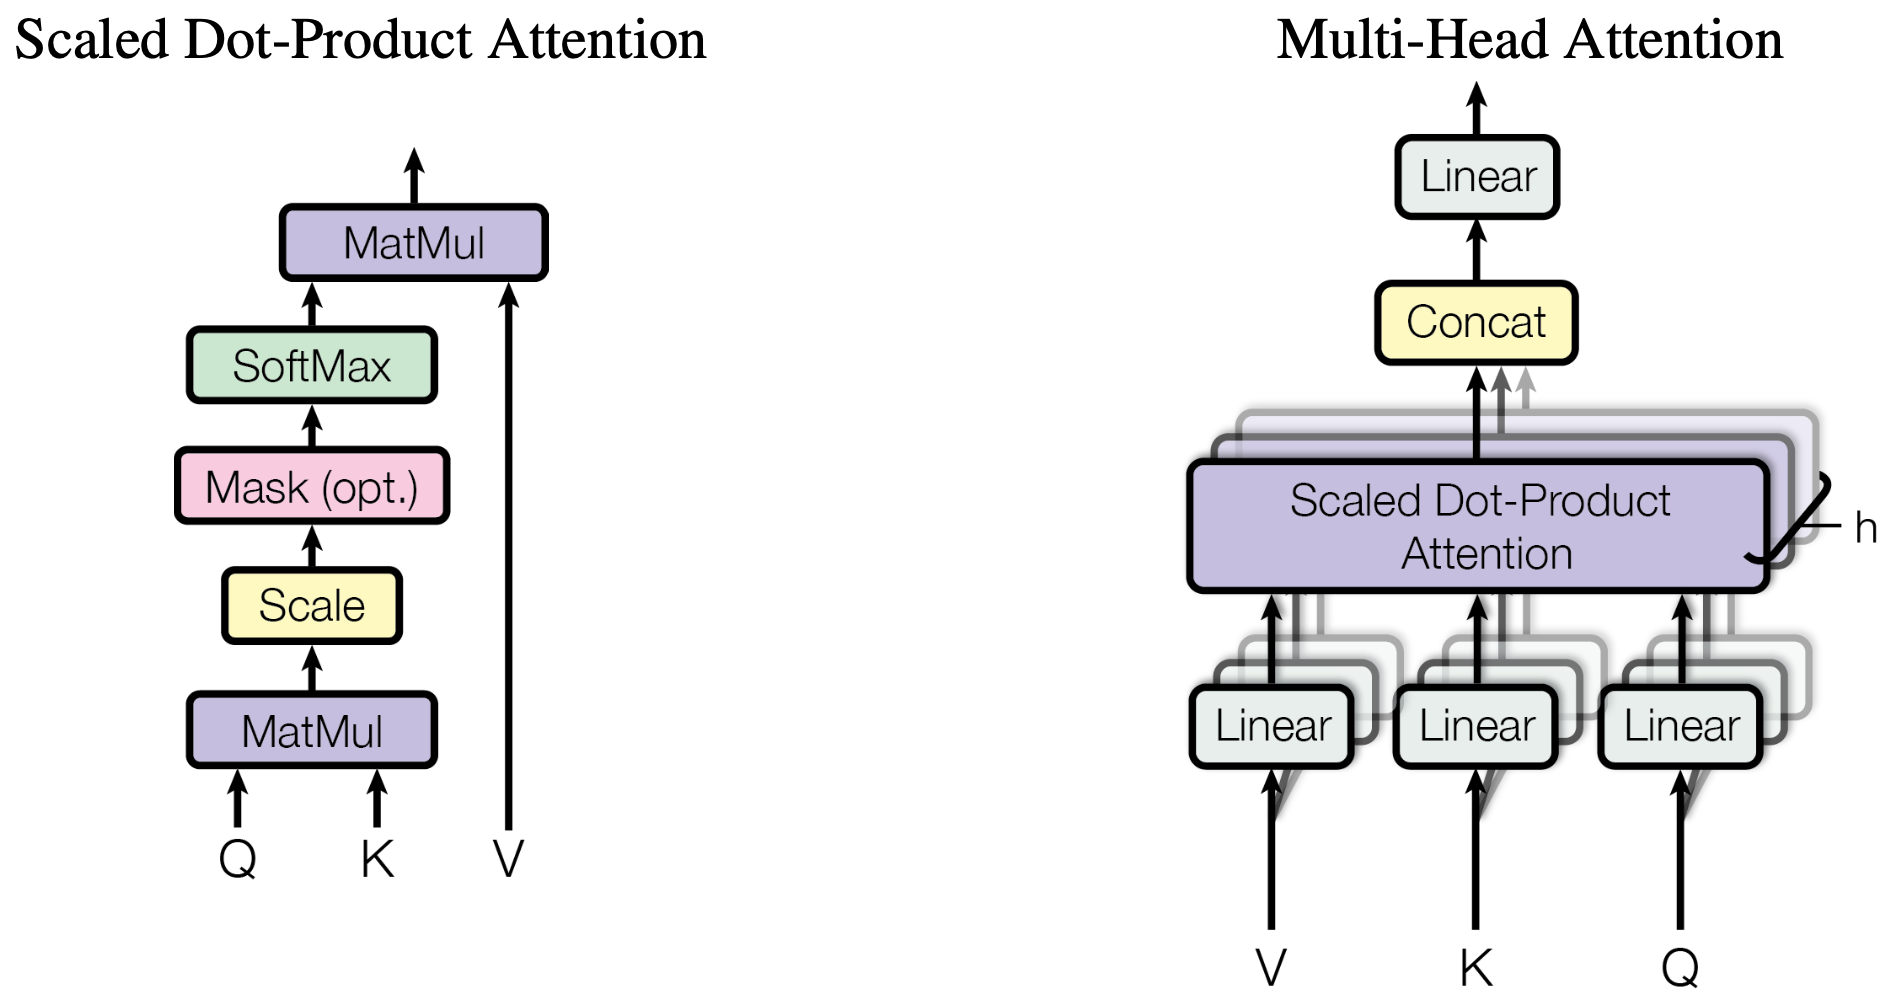
\includegraphics[width = 0.8\textwidth]{figures/attention.png}
	\caption[Scaled Dot-Product Attention and Multi-Head Attention]
	{ (left) Scaled Dot-Product Attention. (right) Multi-Head Attention consists of several attention layers running in parallel. (Image source:~\cite{vaswani2017attention}.)}
	\label{fig:attention}
\end{figure}

\subsection{Multihead Attention}

Multi-head attention allows the model to attend to different representation subspaces at different positions and therefore process richer information. The queries, keys and values are linearly projected h times with different, learned linear projections to dk, dk and dv dimensions respectively. On each of these projections the attention function is computed in parallel, resulting in dv dimensional output values. These are concatenated and projected to obtain the final values, as depicted in Figure 2.3.

\begin{equation}
	\begin{aligned}
MultiHead(Q,K,V) = Concat(head_1,...,head_h)W^O, \\
where \ head_i = Attention(QW_i^Q,KW_i^K,VW_i^V)
\end{aligned}
\end{equation}

\subsection{Positional Encoding}
In the case of RNNs, we feed the words sequentially to the model, each token is aware of how it was ordered. However, multi-head attention computes the output of each item in the sequence independently with no notion of word order. It is inef- ficient to model the sequence information without any special order or position. To account for the order of the words in the input sequence, the Transformer model adds a vector to each input embedding called Positional Encoding. Positional Encoding from the Transformer model is computed by sine and cosine functions of different frequencies as 
\begin{equation}
	\begin{aligned}
	PE_{(pos,2i)} = sin(pos/10000^{2i/d_{model}}),\\
	PE_{(pos,2i+1)} = cos(pos/10000^{2i/d_{model}})
	\end{aligned}
	\label{equ:position_embedding}
\end{equation}

\subsection{The Overall Model Architecture}
The Transformer model with its encoder and decoder components is illustrated in Figure 11. Both Encoder and Decoder are composed of multiple identical encoders and decoders that can be stacked on top of each other Nx times. The encoder stack and the decoder stack share the same number of Nx.

Encoder: The encoder block is a stack of Nx identical layers. Each layer has a multi-head self-attention mechanism sub-layer followed by a position-wise fully connected feed-forward network sub-layer. There are two on each floor sub-layer, the first is a multi-head self-attention mechanism, and the second is a simple feed-forward network with fully connected locations. The residual structure ~\cite{He_2016_CVPR} (see figure ~\ref{fig:transformer})is used on both sub-layers, and finally layer normalization ~\cite{ba2016layer}. That is, the output of each sub-layer is $LayerNorm(x + Sublayer(x))$, where $Sublayer(x)$ is the function implemented by the sub-layer itself. Since the model does not contain any recurrence and convolution, an embedding must be added to the input so that the model can be used in order of the sequence.

The input received by an encoder is a list of vectors, it will input the list of vectors to the self-attention layer, then pass through the feed-forward neural network layer(FFN), and finally get the output, which is passed to the next encoder. The word at each position passes through the self-attention layer, and each output vector obtained passes through the FFN separately, and the feed-forward neural network through each vector is the same.


Decoder: The decoder block is also a stack of Nx identical layers. In addition to the two sub-layers in each encoder layer, the decoder has an extra Masked Multi-Head Attention sub-layer to avoid this attention sub-layer looking into the future.


\section{Faster RCNN}

Faster R-CNN is an advanced network for object detection and the cornerstone for the visual relationship detection models. Compared with other object detection models, Faster R-CNN performs well on localizing and classifying the objects in images. Therefore, it is used as the backbone of object detection in many works about visual relationship detection [1, 20]. Faster R-CNN contains four parts: convolutional layers, region proposal network (RPN), ROI pooling and classifier. In visual relationship detection, the first three parts are utilized to extract the feature map and localize the bounding boxes of objects. The classifier of Faster R-CNN is generally replaced by the advanced model which is designed for visual relationship detection. The structure of Faster R-CNN is illustrated in Fig.~\ref{fig:fasterrcnn}.

\begin{figure}[!htbp]
	\centering
	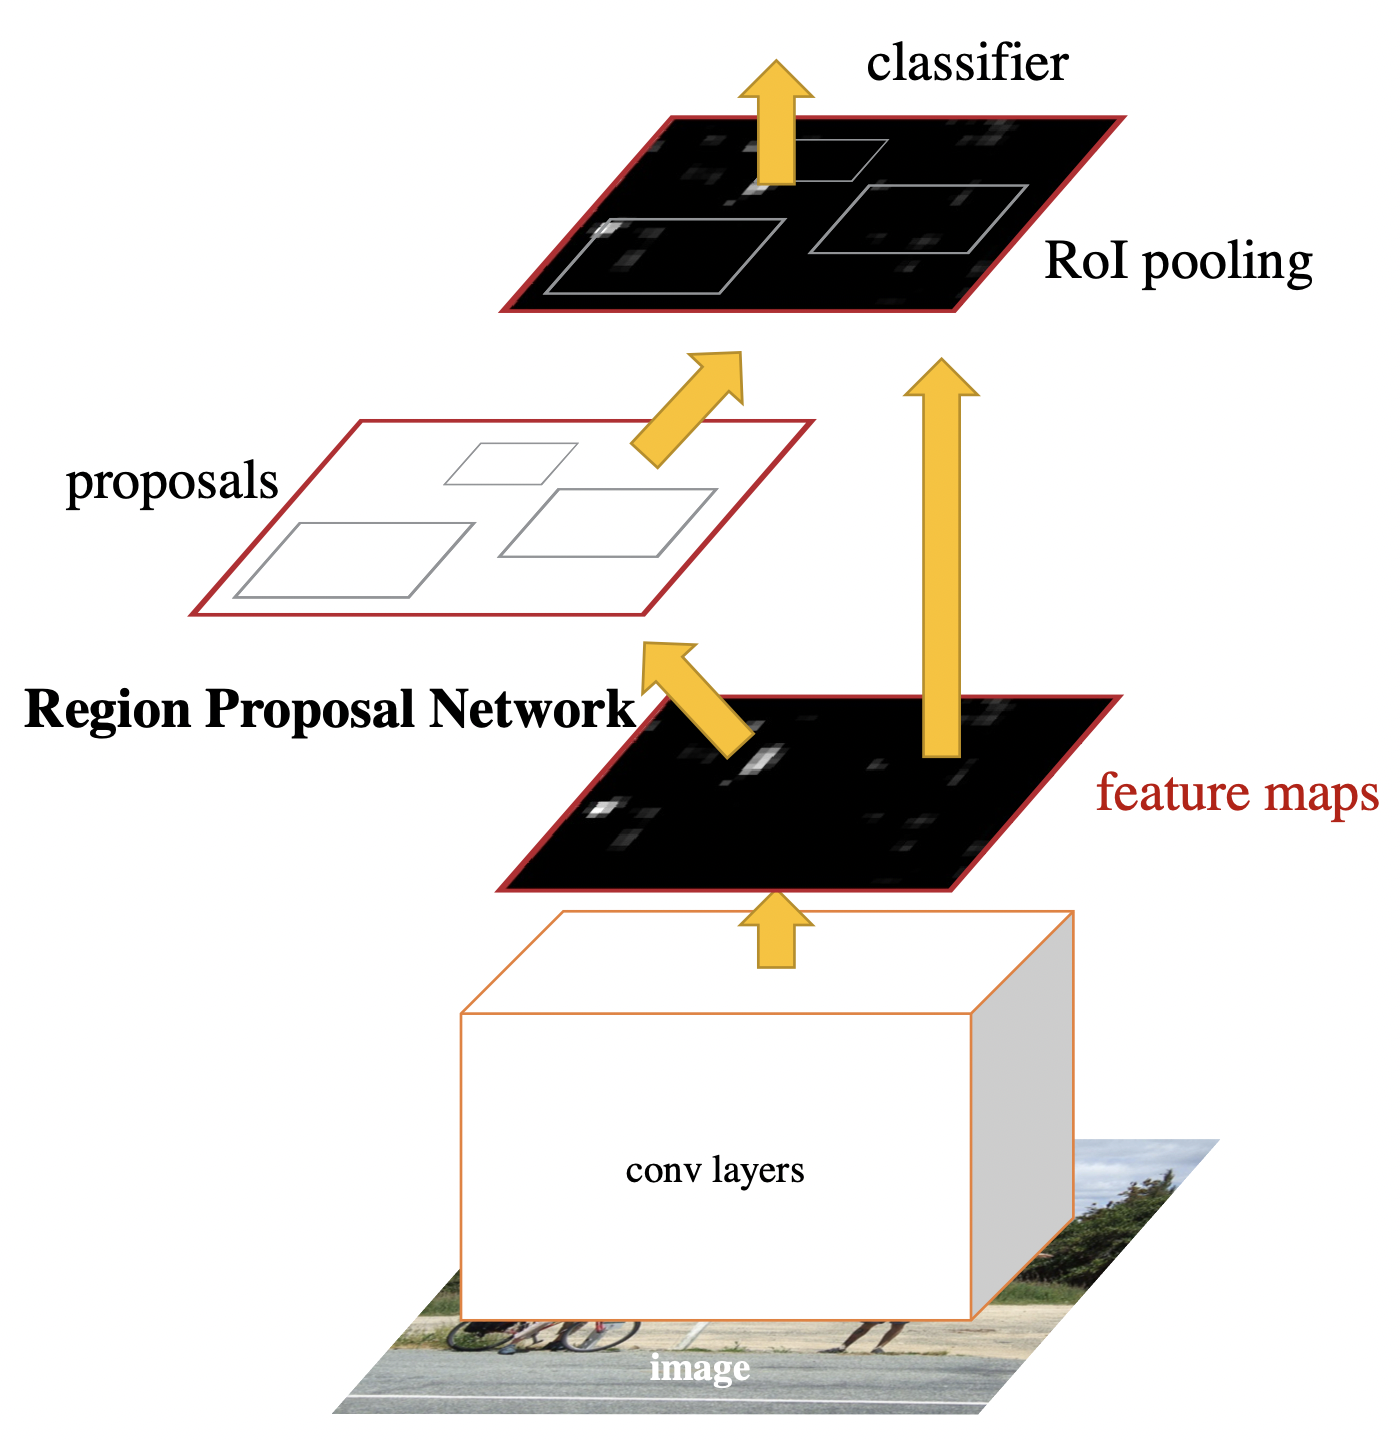
\includegraphics[width = 0.8\textwidth]{figures/fasterrcnn.png}
	\caption[The architecture of Faster R-CNN]
	{ The architecture of Faster R-CNN.}
	\label{fig:fasterrcnn}
\end{figure}

\label{sec:roialign}
\section{ROI Align}
ROI Align is a regional feature aggregation method proposed in the Mask-RCNN~\cite{he2018mask} paper, which solves the problem of regional mis-alignment caused by two quantizations in the ROI Pooling operation. Experiments show that replacing ROI Pooling with ROI Align in the detection task can improve the accuracy of the detection model.

\begin{figure}[!htbp]
	\centering
	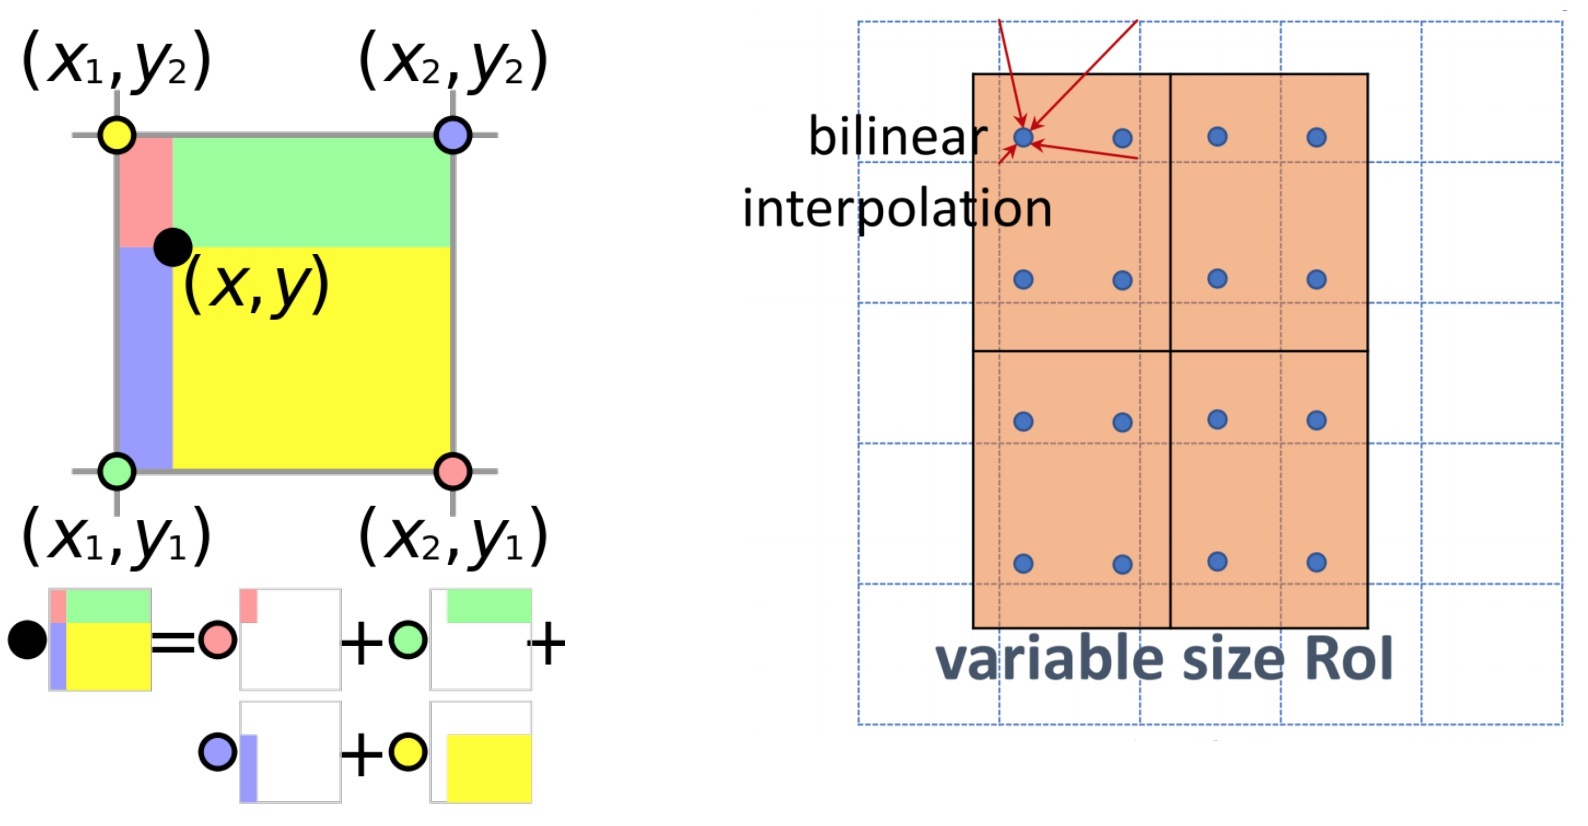
\includegraphics[width=1\linewidth]{figures/roi_align}
	\caption[Bilinear interpolation for ROI Align]{Bilinear interpolation for ROI Align.}
	\label{fig:roialign}
\end{figure}

ROI Align does not need to perform rounding operations like ROI pooling. If the decimal number is calculated, that is, it does not fall on the real pixel, then use the nearest pixel to perform bilinear interpolation on this virtual pixel to get this `pixel'  Value.The step are processed as follow:

\begin{enumerate}[1.]
	\item Divide the bbox area into equal parts according to the size required by the output. It is likely that the vertices will not fall on the real pixels after the equal division.
	\item If the vertices do not fall on the real pixel points after equal division, then take a fixed 4 points in each bin, which is the blue point on the right side of Figure~\ref{fig:roialign}.
	\item For each blue point, the value of the 4 nearest real pixel points is weighted (bilinear interpolation) to obtain the value of this blue point
	\item  4 new values are calculated in a bin, and max is selected from these new values as the output value of this bin Therefore we use bilinear interpolation to predict its value.
	\item Get the final 2x2 output.
\end{enumerate}



\section{Hungarian matching}

Hungarian matching is binary matching using the Hungarian algorithm, it is also a maximum matching. The purpose of maximum matching is to match an edge for each node as much as possible, and the match with the largest number of edges is the maximum match. Usually, in binary matching, each node can only match one edge.

The basic steps of the Hungarian algorithm are as follows:
\begin{enumerate}[1.]
	\item Subtract the smallest entry in each row from all the other entries in the row. This will make the smallest entry in the row now equal to 0.
	\item Subtract the smallest entry in each column from all the other entries in the column. This will make the smallest entry in the column now equal to 0
	\item Draw lines through the row and columns that have the 0 entries such that the fewest lines possible are drawn.
	\item  If there are nn lines drawn, an optimal assignment of zeros is possible and the algorithm is finished. If the number of lines is less than nn, then the optimal number of zeroes is not yet reached. Go to the next step.
	\item Find the smallest entry not covered by any line. Subtract this entry from each row that is not  crossed out, and then add it to each column that is crossed out. Then, go back to Step 3.
\end{enumerate}


\section{Ranking Loss}

Different from Cross-Entropy Loss ~\cite{Categorical_Loss} or Mean Square Error Loss(MSE) ~\cite{CHRISTOFFERSEN2004291}, their goal is to characterize the difference between the output of the model and the actual output. But ranking loss is actually a kind of metric learning, the relative distance they learn does not care about the actual value. Because there are different names in different scenes, including Contrastive Loss, Margin Loss, Hinge Loss or Triplet Loss.

Ranking loss is widely used, including two categories, such as face recognition, which is a person not a person.

\begin{figure}[!htbp]
	\centering
	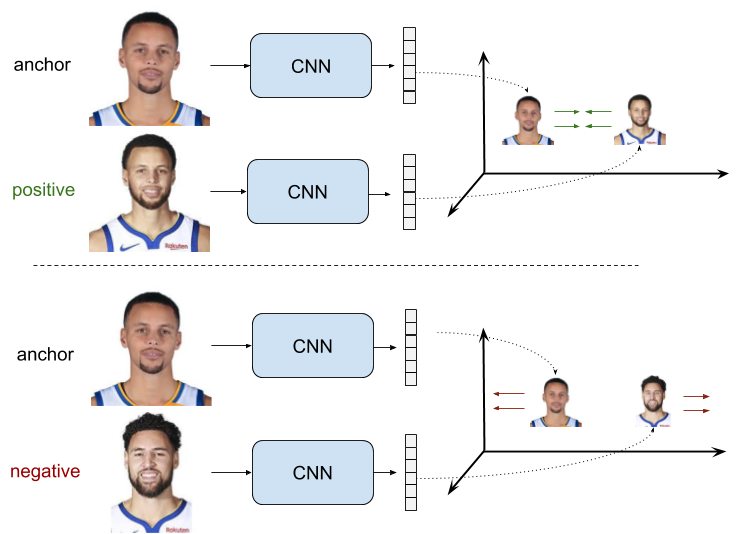
\includegraphics[width = 0.8\textwidth]{figures/pairwise_ranking_loss_faces.png}
	\caption[Example of a pairwise ranking loss ]
	{ Example of a pairwise ranking loss setup to train a net for image face verification. In this setup, the weights of the CNNs are shared. We call it siamese nets. But a pairwise ranking loss can be used in other setups, or with other nets.(Image source:~\cite{triplet_loss_em}.)}
	\label{fig:pairwise_ranking_loss}
\end{figure}


The objective is to learn representations with a small distance $d$ between them for positive pairs, and greater distance than some margin value $m$ for negative pairs. Pairwise Ranking Loss forces representations to have $0$ distance for positive pairs, and a distance greater than a margin for negative pairs. Being $r_a$ and $r_p$the samples representations and $d$ a distance function, we can write:

\begin{equation}
L=\begin{cases}
	d(r_a,r_p) & if \qquad positive\ pair \\
	max(0,m-d(r_a,r_p)) & if \qquad negative\  pair
\end{cases}
\end{equation}

Suppose $r_0,r_1 $ is used to represent the representation of the two elements of the sample, $y$is a two-valued value, when the input is a negative sample pair, it is 0, when a positive sample pair is input, it is 1, and the distance $d$ is Euclidean distance , We can have the final loss function expression:

\begin{equation}
L(r_0,r_1,y)=y\left || r_0-r_1 \right || + (1-y)max(0,m-\left || r_0-r_1 \right ||)
\end{equation}

This setup outperforms the former by using triplets of training data samples, instead of pairs. The triplets are formed by an anchor sample $x_a$, a positive sample $x_p$ and a negative sample $x_n$. The objective is that the distance between the anchor sample and the negative sample representations $d(r_a,r_n)$ is greater (and bigger than a margin $m$) than the distance between the anchor and positive representations $d(r_a,r_p)$. With the same notation, we can write:

\begin{equation}
L(r_a,r_p,r_n)=max(0,m+d(r_a,r_p)-d(r_a,r_p))
\label{equ:ranking_loss}
\end{equation}

\begin{figure}[!htbp]
	\centering
	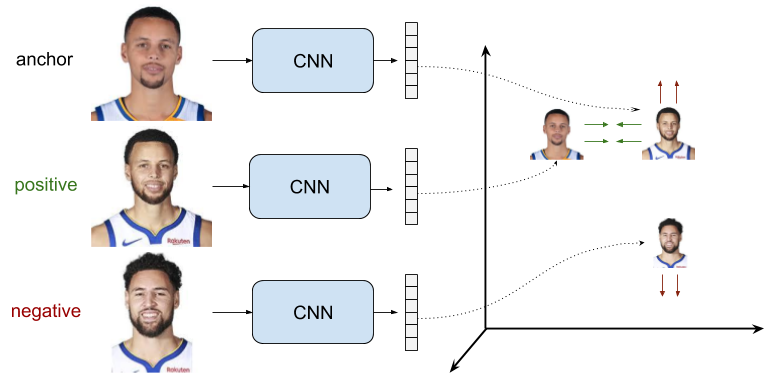
\includegraphics[width = 0.8\textwidth]{figures/triplet_loss_faces.png}
	\caption[Example of a triplet ranking loss ]
	{ Example of a triplet ranking loss setup to train a net for image face verification. In this setup, the weights of the CNNs are shared. We call it triple nets. (Image source:~\cite{triplet_loss_em}.)}
	\label{fig:triplet_ranking_loss}
\end{figure}


\section{Word Representation}

Same as location information, semantic information also helps a lot for understanding relations. The basic encoding method is one hot code. 

One-hot representation is another natural approach to represent words, which assigns a unique index to each word. It is also not good enough to represent words with one-hot representation. First, one-hot representation could not capture the semantic relatedness among words. Second, one-hot representation is a high-dimensional sparse representation, which is very inefficient. Third, it is very inflexible for one-hot representation to deal with new words, which requires assigning new indexes for new words and would change the dimensions of the representation. The change may lead to some problems for existing NLP systems.

Recently, distributed word representation approaches are proposed to address the problem of one-hot word representation. The distributional hypothesis ~\cite{bojanowski2017enriching} that linguistic objects with similar distributions have similar meanings is the basis for distributed word representation learning. Based on the distributional hypothesis, various word representation models, such as CBOW and Skip-gram, have been proposed and applied in different areas.


\begin{figure}[!htbp]
	\centering
	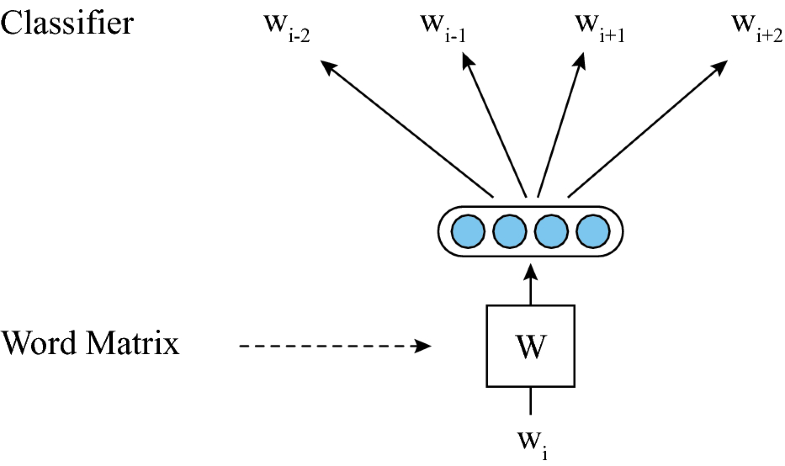
\includegraphics[width = 0.8\textwidth]{figures/skip-gram-model.png}
	\caption[The architecture of skip-gram model]
	{ The architecture of skip-gram model.}
	\label{fig:skip-gram-model}
\end{figure}

One of the widely used distributed word representation is Skip-Gram model (see figure~\ref{fig:skip-gram-model}) which is part of the \textbf{Word2Vec} library. It was created by a team of researchers led by Tomas Mikolov at Google. The main idea is to represent words by means of its neighbors. It tries to predict all neighboring words(the context) of a given word. According to paper~\cite{mikolov2013distributed}, the objective of model is defined as follows:$$\frac{1}{T}\sum_{t=1}^{T}\sum_{-c\le j\le c,j\ne 0} \log_{ p(w_{t+j}\mid w_t) }$$
where w is training word and c is the size of context. So its objective is to find word representations that can predict surrounding words.

Another member of distributed word representations is \textbf{Global Vectors for Word Representation(GloVe)} which is an abbreviation for Global Vectors. While Word2Vec captures certain local context window, GloVe exploits overall co-occurrence statistics of words from corpus, which is a large collection of texts. It consists of two important steps. First one constructs a matrix of term co-occurrences. For each word we compute conditional probability, e.g. for word water $ P(k\mid water) $, where $ k $ is word from vocabulary. If $ k $ is stream, the value of $ P $ is high, and if $ k $ is fashion, then expected value is low as they do not usually co-occur together. After performing all statistical computations, the large matrix is formed. Then high-dimensional context matrix is reduced by normalizing counts and log-smoothing.


\section{VGG16}

\begin{figure}[!htbp]
	\centering
	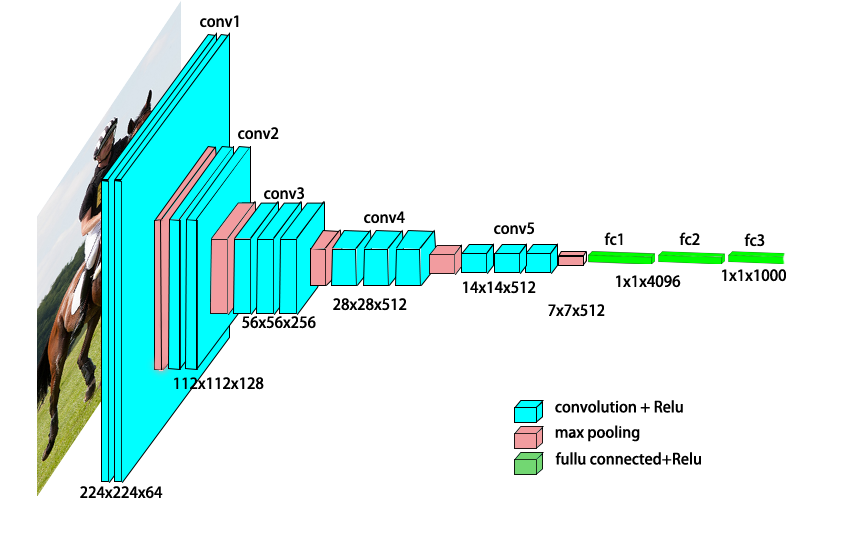
\includegraphics[width=0.8\linewidth]{figures/vgg16}
	\caption[The Architecture of VGG-16]{The Architecture of VGG-16.Image source from~\cite{vgg16img}.}
	\label{fig:vgg16}
\end{figure}
